\documentclass{isprs} 
\usepackage{subfigure}
\usepackage{setspace}
\usepackage{geometry}
\usepackage{epstopdf}
\usepackage[labelsep=period]{caption}  
\usepackage[british]{babel} 


\usepackage{natbib}
\usepackage{amsfonts,amsmath,bm,bbm}
\usepackage{hyperref} 
\usepackage{graphicx,url}
\usepackage{rotating}

\geometry{a4paper, top=25mm, left=20mm, right=20mm, bottom=25mm, headsep=10mm, footskip=12mm}

%\usepackage{isprs}
%\usepackage[perpage,para,symbol*]{footmisc}

%\renewcommand*{\thefootnote}{\fnsymbol{footnote}}
\captionsetup{justification=centering,font=normal} 
\captionsetup[figure]{font=small}
%\captionsetup[table]{font=small} 

\begin{document}
	
	\title{WEIGHTED AMPLITUDE TRANSITION GRAPH: CHARACTERIZATION OF SAR IMAGES}
	
	\author{
		Eduarda T.\ C.\ Chagas\textsuperscript{1}, 
		Alejandro C.\ Frery\textsuperscript{2}, 
		Heitor S.\ Ramos Filho\textsuperscript{1}, 
		Osvaldo A.\ Rosso\textsuperscript{2}
		\thanks{Corresponding author}}
	
	\address{
		\textsuperscript{1 }Dept.\ of Computer Science, Federal University of Minas Gerais, Belo Horizonte, Minas Gerais - (eduarda.chagas, ramosh)@dcc.ufmg.br,\\
		\textsuperscript{2 } Computing Institute, Federal University of Alagoas, Maceió, Alagoas - acfrery@laccan.ufal.br\\
		%Falta o e-mail do professor Rosso
	}
	
	% If the corresponding author is NOT the final author, always add a % space before the subsequent comma, i.e.
	% first author name\textsuperscript{a,}\thanks{Corresponding author} , % second author name \textsuperscript{b}, etc.
	
	
	\commission{VI, }{VI} %This field is optional.
	\workinggroup{VI/4} %This field is optional.
	\icwg{}   %This field is optional.
	
	% KAO: Use times symbol
	\abstract{
		In this paper, we propose a modification of the ordinal pattern transition graph to characterize different types of synthetic aperture radar (SAR) image regions.
		The main justification for the use of such a proposal lies in the difference in the intensity of SAR image data from different target types, due to the backscatter properties.
		Thus, focusing on this problem, we use an ordinal pattern transition graph weighted by the amplitude of the data in the characterization of SAR images.
		In the first step, we use space-filling curves to linearize the HH band data of the image, transforming it into a time-series.
		Soon after, we normalized the received data by rescaling it to the $ [0-1] $ range, since we want to generate a comparability metric between different images.
		In the second step, we apply the weighted amplitude transition graph and extract the probability distribution from the ordinal patterns of the time series.
		Finally, we characterize the regions using causal descriptors of Information Theory.
		Experimental imaging results from Munich urban areas, Guatemala forest regions, and Cape Canaveral ocean regions demonstrate the effectiveness of our technique, which achieves a satisfactory level of separability in the HC Plan when we use patterns with embedding size $m = 3$.
	}
	
	\keywords{Synthetic Aperture Radar (SAR), Time-series, Terrain Classification, Permutation Entropy, Ordinal Patterns Transition Graphs, Causality Complexity-Entropy Plane}
	%Keywords (6--8 words)
	
	\maketitle
	
	%\saythanks % added 28-02-2014 Markus Englich
	
	\section{INTRODUCTION}\label{Intro}
	
	% KAO: Sloppy spacing ensures non-overfull lines. Can be removed if this is not an issue.
	\sloppy
	
	Surface classification and land use are the most important synthetic aperture radar (SAR) imaging applications~\citep{Pottier2004Unsupervised}.
	Supervised and unsupervised classification algorithms have been proposed for this utility~\citep{Bhattacharya2018Unsupervised,Chen1996multifrequency,ZYL1992Bayesian} and previous algorithms have also used the statistical characteristics of the data in the classification process~\citep{Lee1992Wishart}.
	An alternative approach is to use the characteristic information inherent in physical scattering mechanisms.
	SAR image data is sensitive to the dispersion mechanism and is influenced by the shape, orientation and dielectric properties of targets.
	The polarimetric scattering characteristics of different surface types have been thoroughly investigated by~\cite{Moriyama2004study, Fujita2004Polarimetric}.
	Therefore, we will use the amplitude difference information presented in the different surface regions in the ordinal pattern transition graph to perform their respective characterizations.
	
	Given the current methods that provide us with information about the ordinal structure of the series, recent work suggests a weighting in calculating relative frequencies for ordinal patterns with different amplitude variations, making them contribute differently to the final value of permutation entropy ( PE) and thus incorporate amplitude change information within a given data set~\citep{Fadlallah2013Weightedpermutation}.
	
	However, analyzing the current methods we still realize that they do not consider the amplitude difference present in different time series, weighing them in a similar way when calculating the final value of their probabilities.
	Therefore, data with different amplitudes but with similar variance dynamics are not discriminated, losing important information about the system dynamics.
	
	To counterbalance these facts, we propose a modification of the current ordinal pattern transition graph procedure to incorporate meaningful time-series information, with the main motivation of saving useful amplitude information carried by the signal.
	
	We evaluated our technique by proposing a new methodology for characterization of regions in \texttt{SAR} image textures.
	When receiving a texture we perform the linearization process applying \textit{space filling curves} transforming it into a time series, and through the proposed weighted amplitude transition graph we use the discriminatory power of the Information Theory descriptors (permutation entropy and statistical complexity) to perform the characterization of different regions.
	
	The article was divided as follows:
	In the~\ref{OP} section, we introduce the concept of symbolization in ordinal patterns in time series, describing the Bandt-Pompe;
	in the~\ref{OPTG} section, we present the ordinal pattern transition graphs;
	In the~\ref{WATG} section, we propose our technique of ordinal amplitude transition graph weighting by amplitude;
	In the section~\ref{HC}, we report the descriptors of the Information Theory used throughout this work;
	in the~\ref{SAR} section we show the results obtained in characterizing regions in images \texttt{SAR};
	and finally in the~\ref{Conclusion} section, we complete the work.
	
	\section{ORDINAL PATTERNS REPRESENTATIONS -- (OP)}\label{OP}
	
	The representation by ordinal patterns was introduced by~\cite{Bandt2002Permutation}, being used as a method to measure the degree of complexity of data from time series using information theory descriptors.
	As a non-parametric method, Bandt-Pompe's formation of ordinal patterns consists of a simple approach, resistant to noise contamination effects, invariant to linear and nonlinear monotonic transformations and, considering the temporal causality of the data, reveals important details of the ordinal structure of the time series~\citep{Larrondo2006Random}.
	
	Let the finite time series of discrete time real values $\mathbb{X} = (x_1, x_2, \dots, x_T)$ with length $T$.
	The $\mathbb{X}_t^{m, \tau} $ symbols or words performed at each instant $t = 1, \dots, T- (m-1) \tau$ are given by an embedding dimension $m \in \mathbb{N}$ and time delay $\tau \in \mathbb{N}$ between patterns:
	
	\begin{equation}
	\mathbb{X}_t^{m,\tau} = (x_{(t-1)+\tau}, x_{(t-1)+\tau+1},\ldots, x_{(t-1)+\tau+(m-1)}).
	\end{equation}
	
	The set of ordinal patterns $\pi = \{\pi_t^m: t = 1, \dots, T- (m-1) \tau \}$ are obtained by mapping $\mathbb{X}^{m, \tau}_t \mapsto \pi^m$ realized through the permutation process of the elements, such that they are ordered in increasing order ~\citep{Ravetti2014noise}:
	$$x_{(t-1) + \tau} \leq x_{(t-1) + \tau + 1} \leq \ldots \leq x_{(t-1) + \tau + (m-1)}.$$
	
	Since $\Pi$ is the symbol sequence obtained by a given series $\mathbb{X}_t^{m,\tau}$, the Bandt-Pompe probability distribution is the relative frequency of symbols in the series against $m!$ possible permutations of patterns $\{\pi_t^m \}_{t = 1}^{m!}$:
	
	\begin{equation}
	p(\pi_i^m) = \frac{\#\left \{t : t = 1, \dots, T-(m-1)\tau; \mathbb{X}_t^{m,\tau} \text{ type } \pi_i^m\right \}}{T- (m-1)\tau},  
	\end{equation}
	
	that meets the conditions $p(\pi_i^m) \ge 0$ and  $\sum_{i=1}^{m!} p(\pi_i^m) = 1$.
	
	\section{ORDINAL PATTERNS TRANSITION GRAPH -- (OPTG)}\label{OPTG}
	
	Seeking to extract intrinsic characteristics from time series generator phenomena, the ordinal pattern transition graphs appear as an additional step in the non-parametric analysis by information theory descriptors.
	
	The graph $\vec{G}_{\pi} = (\vec{V}, \vec{E})$ indicate the transitions between two consecutive ordinal patterns over time $t$.
	In this new representation, the patterns $\{\pi_t^m \}_{t = 1}^{m!}$ match the vertices of the set $\vec{V} = \{v_{\pi_i}: i = 1, \dots, m! \}$ and the edges $\vec{E} = \{(v_{\pi_i}, v_{\pi_j}): v_{\pi_i}, v_{\pi_j} \in V \}$ indicate the sequential occurrence of two ordinal patterns in the analyzed data set.
	
	Two approaches are considered in relation to the weight of edges in the literature: some authors employ unweighted edges ~\citep{McCullough2015lagged, Kulp2016ordinal} representing only the existence of such transitions, while others apply the frequency of transitions as ~\citep{Sorrentino2015periodic, Zhang2017ConstructingOP}.
	
	The weights $\mathbb{W} = \{w_{v_{\pi_i}, v_{\pi_j}}: v_{\pi_i}, v_{\pi_j} \in V \}$ assigned to each edge describes the chances of transition between two particular patterns $(v_{\pi_i}, v_{\pi_j})$ calculated by their respective relative frequencies, ie:
	
	\begin{equation}
	w_{v_{\pi_i}, v_{\pi_j}} = \frac{|\Pi_{\pi_i,\pi_j}|}{m-1},
	\end{equation}
	
	on what $|\Pi_{\pi_i,\pi_j}|$ is the number of transitions from pattern $\pi_i$ to pattern $\pi_j$ and $\sum_{v_{\pi_i}, v_{\pi_j}}w_{v_{\pi_i}, v_{\pi_j}} = 1$.
	
	\section{WEIGHTED AMPLITUDE TRANSITION GRAPH -- (WATG)}\label{WATG}
	
	We refer to this procedure as Weighted Amplitude Transition Graph (WATG) and summarize in the following steps.
	
	First, each $\mathbb{X}$ time series will be resized and scaled to within the $[0, 1]$ range, since we are generating a comparability metric between different data sets.
	Thus, for this we use the following normalization process:
	
	\begin{equation}
	x_{new} = \frac{x - x_{min}}{x_{max} - x_{min}}
	\end{equation}
	
	
	Each $\mathbb{X}^{m, \tau}_t$ vector will be associated with a $\beta_t$ weight value, indicating its amplitude.
	This value will be given by the largest difference between its elements, as we can see below:
	
	
	\begin{equation}
	\beta_t = \max\{x_i - x_j\},
	\end{equation}
	on what $x_i, x_j \in \mathbb{X}^{m, \tau}_t$.
	
	Traditionally, the transition graph assigns uniform weight to each transition between patterns and normalizes the result obtained by dividing by the total transitions.
	In this modification, the $w_{v_{\pi_i}, v_{\pi_j}}$ weights assigned to each edge depict the amplitude difference observed in the transition.
	So we have to:
	
	\begin{equation}
	w_{v_{\pi_i}, v_{\pi_j}} =  \sum_{i : \{\mathbb{X}^{m,\tau}_t \mapsto \pi_i\}} \sum_{j : \{\mathbb{X}^{m,\tau}_t \mapsto \pi_j\}} |\beta_i - \beta_j| .
	\end{equation}
	
	Thus, the probability distribution taken from the weighted amplitude transition graph is given as follows:
	
	\begin{equation}
	\left\{\begin{array}{l}
	\lambda_{v_{\pi_i}, v_{\pi_j}} = 1, \text{ se } (v_{\pi_i}, v_{\pi_j}) \in \vec{E} \\
	\lambda_{v_{\pi_i}, v_{\pi_j}} = 0, \text{ caso contrário}.
	\end{array}\right.
	\end{equation}
	
	\begin{equation}
	p(\pi_i, \pi_j) = \frac{\lambda_{v_{\pi_i}, v_{\pi_j}} . w_{v_{\pi_i}, v_{\pi_j}}}{\sum_{v_{\pi_a}, v_{\pi_b}} w_{v_{\pi_a}, v_{\pi_b}}}.
	\end{equation}
	
	Note that the conditions $p(\pi_i, \pi_j) \ge 0$ e $\sum_{\pi_i, \pi_j} p(\pi_i, \pi_j) = 1$ are satisfied.
	
	Thus, series with uniform amplitudes have edges with probability of occurrence well distributed along the graph, while those with small amplitude and large peaks have edges with probability of occurrence much higher than the others.
	
	\section{INFORMATIONAL CAUSAL ENTROPY-COMPLEXITY PLANE}\label{HC}
	
	Entropy measures the disorder or unpredictability of a system characterized by a probability function $\mathbb{P}$.
	
	Let $\mathbb{P} = \{p_{(\pi_1, \pi_1)}, p_{(\pi_1, \pi_2)}, \dots, p_{(\pi_{m!}, \Pi_{m!})} \}$  the probability distribution taken from the time series weighted amplitude transition graph $\mathbb{X}$.
	Shannon's entropy is given by:
	
	\begin{equation}
	H(\mathbb{P}) = -\sum_{i=1}^{m!m!} p_i \log p_i .
	\label{eq:Entropia}
	\end{equation}
	
	Ability of the Entropy to capture system properties is limited, so it is necessary to use it in conjunction with other descriptors to perform a more complete analysis.
	Other interesting measures are distances between the $\mathbb{P}$ probability function and a probability measure that describes a non-informative process, typically uniform distribution.
	
	The Jensen-Shannon distance to the uniform distribution $\mathbb{U} = (\frac{1}{m!m!}, \dots, \frac{1}{m!m!})$ consists of a measure of how similar the underlying dynamics are to a process without any information, being calculated as:
	
	\begin{equation}
	D(\mathbb{P}, \mathbb{U}) = \sum_{i=1}^{(m!m!)} \Big(p_i \log\frac{p_i}{u_i} +
	u_i \log\frac{u_i}{p_i}
	\Big).
	\end{equation}
	
	Conversely to entropy, statistical complexity seeks to find interaction and dependence structures among the elements of a given series, being an extremely important factor in the study of dynamic systems.
	
	This property is defined using the formula developed by Lopèz-Ruiz, Mancini and Calbet, where an Entropy and a Distance, also called an disequilibrium, can be combined in the Statistical Complexity attribute to increase its power of description~\citep{Feldman2008information,Feldman1998Statistical,Lopez1995statistical}:
	
	\begin{equation}
	C(\mathbb{P}, \mathbb{U}) = H(\mathbb{P}) D(\mathbb{P}, \mathbb{U}).
	\end{equation}
	
	Each time series can then be described by a dot $(H(\mathbb{P}), C(\mathbb{P}, \mathbb{U}))$.
	The set of all pairs $(H(\mathbb{P}), C(\mathbb{P}, \mathbb{U}))$ for any time series described by patterns of length $m$ lies in a compact subset of $\mathbbm R^2$: the Entropy-Complexity plane. 
	Through such a tool it is possible to discover the nature of the series, determining if it corresponds to a chaotic, stochastic or deterministic sequence, analyzing its behavior since they have different dynamics.
	
	\section{CLASSIFICATION SAR REGIONS}\label{SAR}
	
	In this work we propose a new image characterization methodology \texttt{SAR}.
	When receiving a texture we perform the linearization process by applying \textit{space filling curves} and using the weighted amplitude transition graph we use the discriminatory power of Information Theory to perform the characterization using the Entropy-Complexity plane in different regions extracted from textures from images \texttt{SAR}.
	
	\textit{Space filling curves} were first seen in~\cite{Nguyen1982SpaceFC}, turning a texture into a one-dimensional signal.
	When used as scanning methods of an image, such functions can well preserve the eminent properties of pixel spatial correlation, while not providing sufficient discriminatory power to classify natural textures~\citep{Lee1994Texture}.
	
	Assuming an image is supported by a $N \times N$ dimension grid, where $N$ is a power of $2$, we have the following definition.
	
	\newtheorem{mydef}{Definition}
	\begin{mydef}
		An image scan is a bijector function $f \colon \mathbb{N} \times \mathbb{N} \to \mathbb{N}$ in the ordered pair set $ \{(i, j): 1 \leq i , j \leq N \}$, which denotes the points in the domain, for the closed range of integers $\{1, \dots, N^2\}$. Equivalently, the image is encoded by scanning $ f $ at pixel intensities in the order $P_{f^{-1}(1)}, P_{f^{-1}(2)}, \dots, P_{f^{-1}(N^2)}$, where $P_{(i, j)}$ represents the pixel strength of column $i$ and row $j$.
		\label{def:CurveFilling}
	\end{mydef}
	
	\textit{Space filling curves}, such as raster-1, raster-2 and Hilbert scanning techniques are characterized by the definition~\ref{def:CurveFilling}, providing a proper function $f$.
	As can also be seen from the definition~\ref{def:CurveFilling}, curves impose on us the condition that each pixel is visited only once.
	In this paper, we pay more attention to the result of the characterization obtained through the \texttt{Hilbert curve}.
	
	Widely used in recognizing geographical features and patterns, synthetic aperture radar (\texttt{SAR}) images are rich in texture information. For this analysis three images \texttt{SAR} with different regions were used, they are:
	
	\begin{itemize}
		\item Sierra del Lacandon National Park, Guatemala (acquired on April 10, 2015), available at \url{https://uavsar.jpl.nasa.gov/cgi-bin/product.pl?jobName=Lacand_30202_15043_006_150410_L090_CX_01#dados};
		\item Cape Canaveral Ocean Regions (acquired September 22, 2016);
		\item Urban area of the city of Munich, Germany (acquired June 5, 2015).
	\end{itemize}
	
	A total of 160 samples were considered during the investigation, 40 samples from each category of regions, namely: Guatemalan forest regions; oceanic regions of Cape Canaveral with behavior 1; oceanic regions of Cape Canaveral with behavior 2 and urban regions of the city of Munich. To further illustrate the generated sample set, Figure~\ref{fig:RegionsSAR} exemplifies each of the present categories.
	
	\begin{figure}[!h]
		\centering
		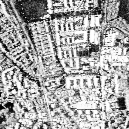
\includegraphics[width=.23\linewidth]{Figures/munichUrban.png}
		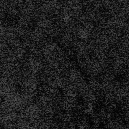
\includegraphics[width=.23\linewidth]{Figures/Cape1.png}
		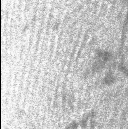
\includegraphics[width=.23\linewidth]{Figures/Cape2.png}
		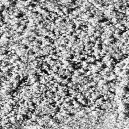
\includegraphics[width=.23\linewidth]{Figures/guatemalaflorest.png}
		\caption{Types of regions analyzed: (a) urban regions; (b) Oceanic Region Type 1; (c) Oceanic Region Type 2 and (d) Forest Regions.}\label{fig:RegioesSAR}
	\end{figure} 
	
	The images used in this experiment are results of the HH \texttt{SAR} band and each sample is represented by a $128 \times 128$ pixel sub-image.
	Since the symbolization process is invariant the Monotonous transformations and resistant to contamination effects, contrast changes are not capable of causing changes in the final results obtained by the descriptors.
	Thus, the different types of oceanic regions considered in this study were studied as a single more general class.
	
	Data resulting from remote sensing have a peculiar feature that justifies the application in this article:
	The intensities of an image and hence the amplitude difference in the data classes depend on the properties of the target we are analyzing due to the backscatter properties.
	Thus, urban targets are those that usually give the highest returns, followed by forests, and finally, water bodies, as can be seen in the figure~\ref{fig:AmplitudeSAR}.
	
	Therefore, in this paper we aim to represent, through the weighted amplitude transition graph, to model this amplitude difference in the probability distribution of our data.
	The analysis methodology proposed and applied to the texture data set \texttt{SAR} can be seen in the figure~\ref{fig:WATG}.
	
	\begin{figure}[hbt]
		%\begin{center}
		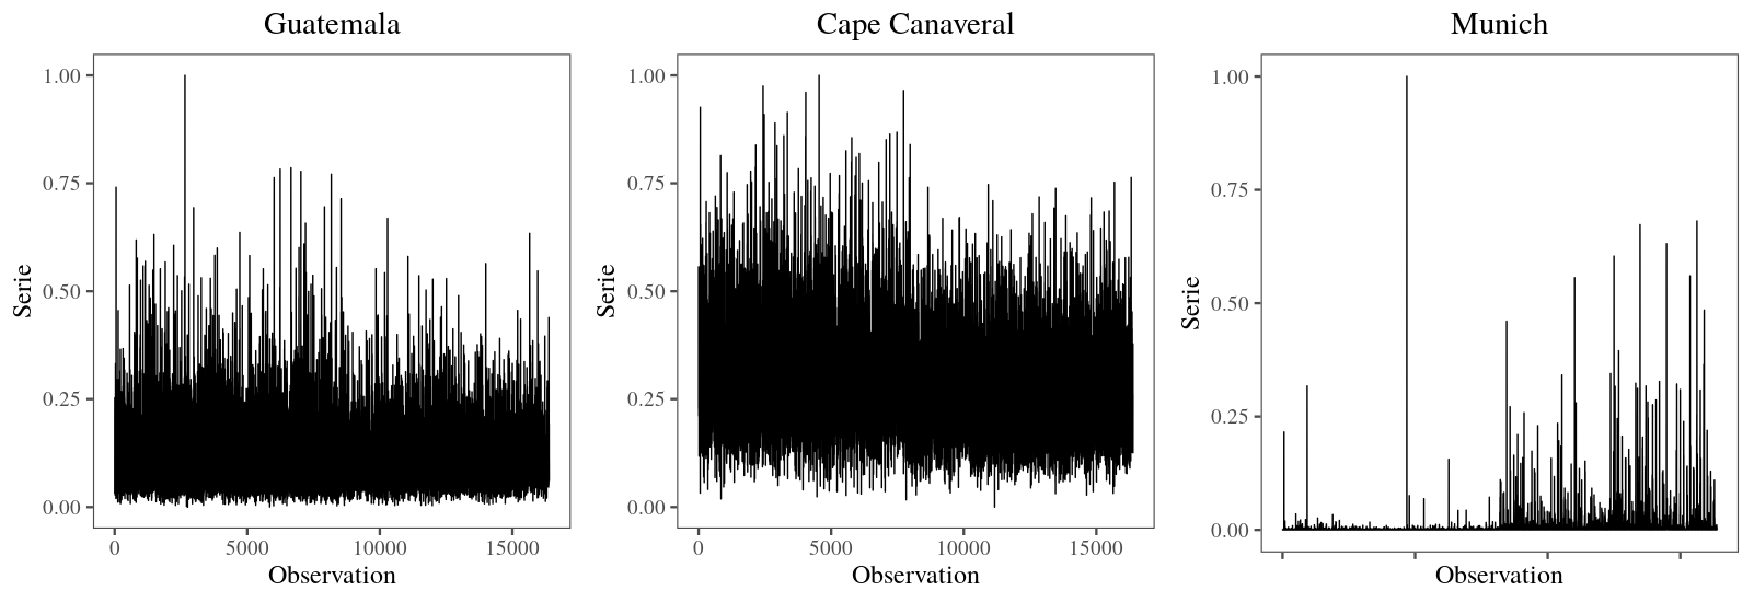
\includegraphics[scale = 0.28]{Figures/SAR_signal.pdf}
		\caption{Analysis of the amplitude of the different types of regions: (a) Oceanic Region; (b) Forest Regions and (c) Urban Regions}
		\label{fig:AmplitudeSAR}
		%\end{center}
	\end{figure}
	
	After linearizing the textures using the Hilbert curve, we used the sliding window technique to obtain our symbols, thus:
	
	\begin{equation}
	\mathbb{X}_t^{m,\tau} = (x_{t}, x_{t+\tau},\ldots, x_{t+(m-2)\tau} ,x_{t+(m-1)\tau}).
	\end{equation}
	
	\begin{figure}[hbt]
		\centering
		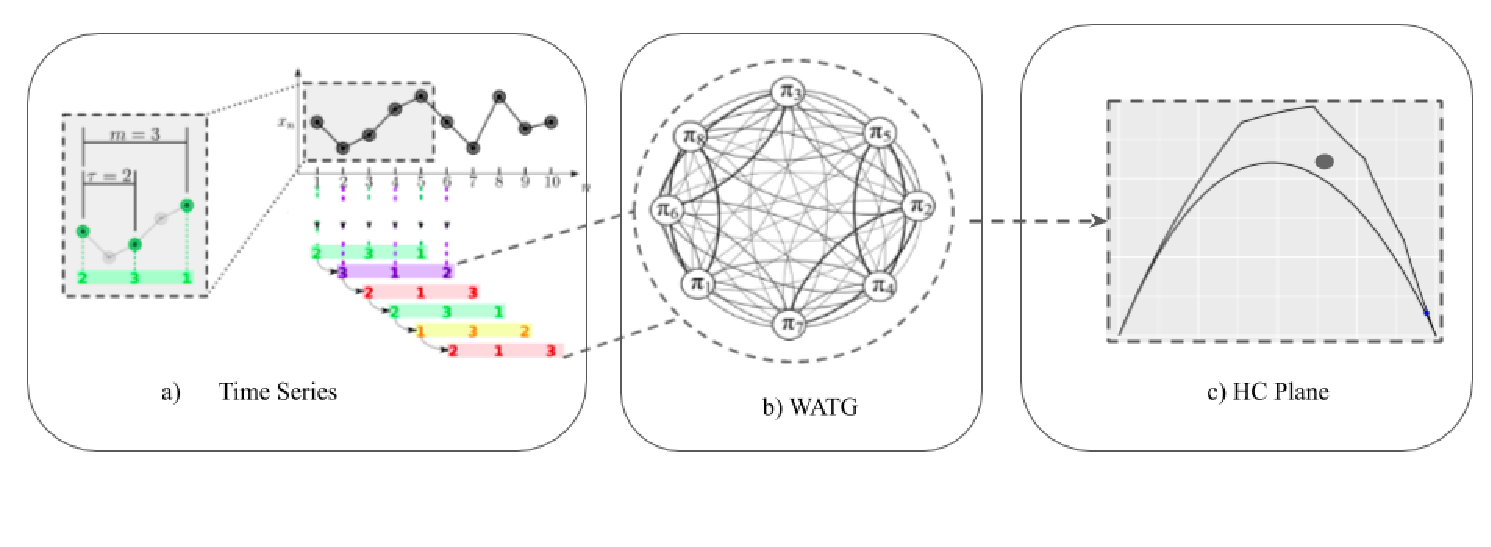
\includegraphics[scale = 0.25]{Figures/WATG.pdf}
		\caption{The methodological process applied in the characterization of regions \texttt{SAR}.}
		\label{fig:WATG}
	\end{figure}
	
	The results achieved can be seen in figure~\ref{fig:Regions}, where we test the power of the technique effect under different dimension values $m$ and delay $\tau$.
	Since such values inform us of intrinsic characteristics of the dynamics of the series in their specific domains, inadequate values may hide this kind of knowledge about the data, and this analysis step is extremely crucial.
	As expected, following the sliding window model, we get better characterization when we apply the delay $\tau = 1$.
	
	\section{CONCLUSION}\label{Conclusion}
	
	In this paper, we propose a new weighting technique in the ordinal pattern transition graph, where we can now not only analyze the amplitude of a given time series but also have a new comparability metric.
	The idea is initially to normalize the data and to assign as edge weights the amplitude variations during the transitions.
	Thus, the closer the entropy $\mathbb{H}$ is to $0$ the more uniform the probability distribution $\mathbb{P}$ will be, informing us that the series does not have large amplitude variances.
	However, if a series has a low amplitude but has large variations (peaks) over time, WATG will be able to infer such behavior by placing a greater weight on these transitions, making the entropy $\mathbb{H}$ approach $1$.
	
	To test the proposed technique we performed the characterization of different regions in textures of images \texttt{SAR}, which due to the backscatter properties in different types of targets, result after linearization, in series with marked amplitude differences.
	
	As a result, in addition to perfectly separating urban areas from the others analyzed by entropy values, we are still able to differentiate oceanic and forest areas through their different values of statistical complexity, which informs us of the degree of temporal dependence between their elements, which now linearized, also informs us about the spatial dependence of our texture.
	
	\bibliographystyle{isprs}
	\bibliography{ISPRS}
	
	\section*{ACKNOWLEDGEMENTS}\label{ACKNOWLEDGEMENTS}
	
	This work was partially funded by the Coordination for the Improvement of Higher Education Personnel (CAPES).
	
	\onecolumn
	\newpage
	\begin{sidewaysfigure}
		\centering
		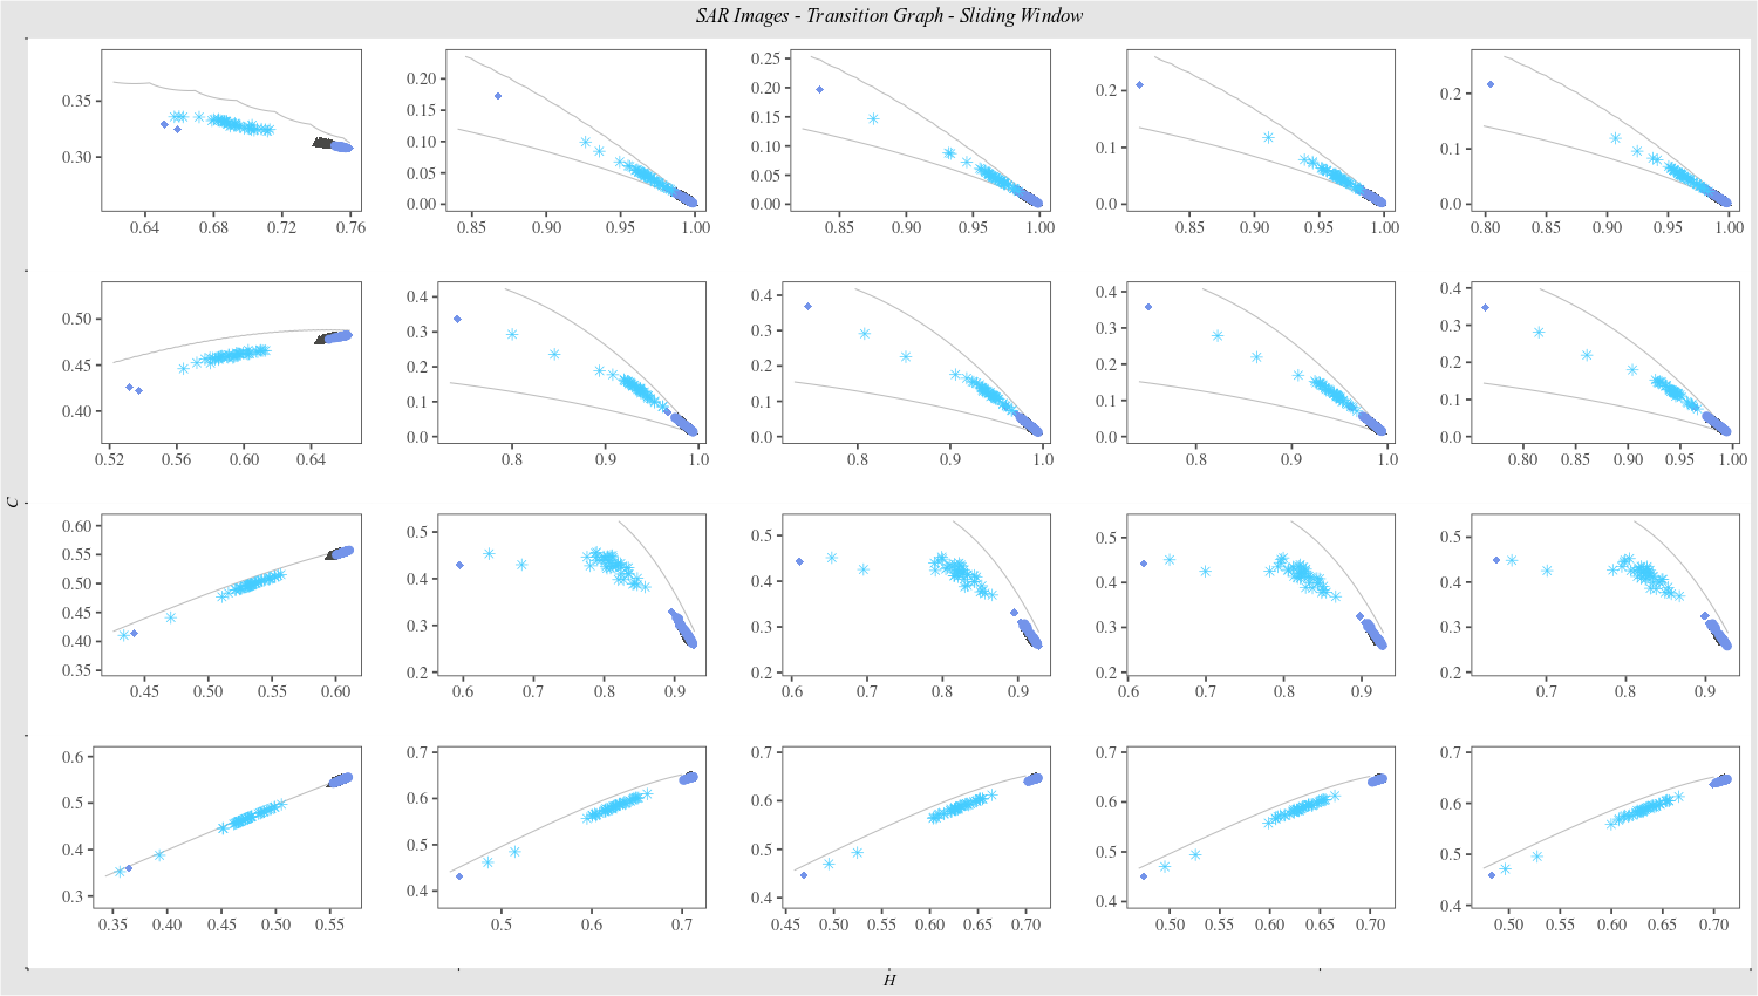
\includegraphics[width=1.05\textwidth]{Figures/transitionGraphHilbert.pdf}
		\caption{Characterization resulting from the application of the \texttt{Hilbert curve} in WATG on textures of different regions: Guatemala (Green), Cape Canaveral (Blue) and Munich (violet). Charts evolve horizontally according to the $m$ dimension chosen and vertically with the delay $\tau$}
		\label{fig:Regions}
	\end{sidewaysfigure}
	
\end{document}
